\documentclass[english]{article}

\makeatletter 
\def\input@path{{../../}} 
\makeatother

\usepackage[T1]{fontenc}
\usepackage[utf8]{inputenc}
\usepackage{float}
\usepackage{graphicx}

%%%Todo lo de arriba viene de lyx y no se que hace

\usepackage{subfiles}						%MULTIARCHIVOS, NO BORRAR

%donde voy a buscar los archivos de imagenes 
\graphicspath{{Ej1/Informe/imagenes/}{Ej1/Informe/}
			  {Ej2/Informe/imagenes/}{Ej2/Informe/}
			  {Ej3/Informe/imagenes/}{Ej3/Informe/}
			  {Ej4/Informe/imagenes/}{Ej4/Informe/}
			  {Ej5/Informe/imagenes/}{Ej5/Informe/}
			  {Ej6/Informe/imagenes/}{Ej6/Informe/}}	
										

\usepackage{nomencl}					%Para introducir nomenclaturas/definciones
\usepackage{makecell}					%Para emprolijar celdas de tablas
\usepackage{amsmath}
\usepackage{amssymb}					%simbolos matematicos
\usepackage{upgreek}					%puedo usar \uptau que es como \tau pero con mas rulito
\usepackage{steinmetz}
\usepackage{mathtools}
\usepackage{placeins}
\usepackage[textwidth=16cm]{geometry}	%texto ocupa mas ancho de pagina
\usepackage{xcolor}						%se usa en \code
\usepackage[american]{circuitikz}		%dibujar esquematicos y diagramas
\usepackage[parfill]{parskip}			%pone espacio entre parrafos
\setlength{\parindent}{10pt}			%cuanta sangria al principio de un parrafo
\usepackage{indentfirst}				%pone sangria al primer parrafo de una seccion
\usepackage{gensymb}
\usepackage{textcomp}
\usepackage{hyperref}
\usepackage{pdfpages}
\usepackage{wrapfig}					%permite figuras envueltas por texto
\usepackage[colorinlistoftodos]{todonotes}	%TODOs
\usepackage{subcaption}					%funciones extras para las subfiguras



% Swap the definition of \abs* and \norm*, so that \abs
% and \norm resizes the size of the brackets, and the 
% starred version does not.
\DeclarePairedDelimiter\abs{\lvert}{\rvert} %
\makeatletter	%magia de categoria de caracteres en Tex, ignorar
\let\oldabs\abs 
\def\abs{\@ifstar{\oldabs}{\oldabs*}}
\let\oldnorm\norm
\def\norm{\@ifstar{\oldnorm}{\oldnorm*}}
\makeatother	%magia de categoria de caracteres en Tex, ignorar

%Definicion comando \parsum: hace re piola el simbolo de la suma en paralelo
\newcommand{\parsum}{\mathbin{\!/\mkern-5mu/\!}} 

%Definicion comando \code: poen el texto en fuente monoespaciada con fondo gris 
%al estilo del codigo de stack overflow
\definecolor{light-gray}{gray}{0.95} 
\newcommand{\code}[1]{\colorbox{light-gray}{\texttt{#1}}}




%cambia las palabras que estan en ingles a castellano
\AtBeginDocument{\renewcommand\contentsname{Índice}}
\AtBeginDocument{\renewcommand\figurename{Figura}}


\makeatletter

\begin{document}

Lorem ipsum dolor sit amet, consectetur adipiscing elit. Pellentesque aliquam facilisis lacus sit amet porttitor. Aliquam in nisi eu nisl accumsan blandit. Vestibulum accumsan dictum justo vitae fringilla. Sed quis felis porta, lacinia urna ut, lobortis mauris. Nullam blandit elementum nulla placerat eleifend. Class aptent taciti sociosqu ad litora torquent per conubia nostra, per inceptos himenaeos. Nunc egestas suscipit sollicitudin. Quisque venenatis, massa at congue gravida, mauris mauris feugiat dui, at egestas mi justo vitae mi. Morbi finibus, ante at efficitur molestie, nibh elit imperdiet mi, eu laoreet dolor quam nec diam. Donec finibus iaculis tristique. Donec mi turpis, tempus vitae ligula in, tincidunt sagittis elit. Aenean a lectus id enim bibendum commodo non a nibh.


\let\oldinput=\input 		%backup del comando input
\def\input#1{\oldinput{Ej1/Informe/#1}}	%aclara donde encontrar cualquier include proximo

\subfile{ej1.tex}	%incluyo nuevo archivo

\let\input=\oldinput	%vuelvo al comando original

%


%\documentclass[../../main.tex]{subfiles}
\begin{document}

\section{Medici\'on corriente de bias y tensi\'on de offset}


\begin{circuitikz}
  		\draw (0,0) node[op amp][yscale=-1] (opamp) {}
  		(opamp.-) 	to[short]($(opamp.-)-(0.5,0)$) 
  					to[short]($(opamp.-)-(0.5, 1.5)$)
  					to[R=$R_1$]($(opamp.-)-(0.5,3)$)
  					node [ground]{}
  		($(opamp.-)-(0.5, 1.5)$) to[R=$R_2$] ($(opamp.-)-(-2.38, 1.5)$)
  					to[short]($(opamp.out)$)
  					
  		(opamp.+) to[short] ($(opamp.+)-(2,0)$)
  				  to[R=$R_3$]($(opamp.+)-(3.5,0)$)
  				  to[sV=$V_{in}$]($(opamp.-)-(3.5,3)$) node[ground]{}
  				  

		($(opamp.+)-(1.5,0)$) to[R=$R_4$] ($(opamp.-)-(1.5,3)$) node[ground] {}
		
		(opamp.out) to ($(opamp.out)+(1,0)$) node[ocirc]{$\,\, V_{out}$}
  		
  		;
\end{circuitikz}



\subsection{Modelo de amplificador operacional con corrientes de bias y tensi\'on de offset}

\begin{figure}[htb]	%modelo opamp vio ibias
	\centering
	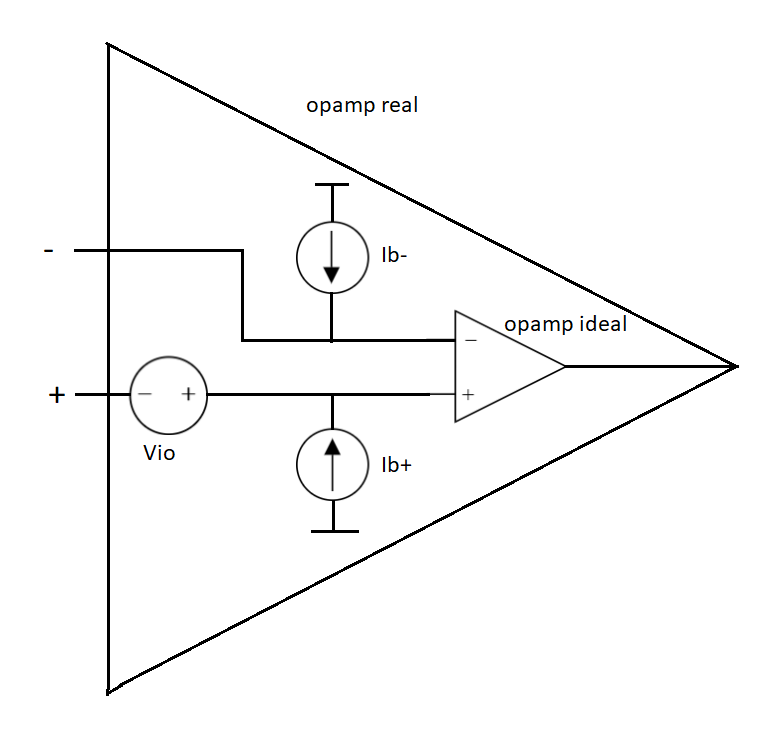
\includegraphics[width=0.4\textwidth]{imagenes/modelo_opamp_vio_ibias.png}
	\caption{Modelo de amplificador operacional con corrientes de bias y tensi\'on de offset}
	\label{fig:ej_3_modelo_opamp_vio_ibias}
\end{figure}

\todo[inline]{Que es corriente de bias y tension de offset. fijarme que puso roch en la intro}











\subsection{Importancia de las corrientes de bias y la tensi\'on de offset}


Las corrientes de bias($I_B^+$ y $I_B^-$) y la tensi\'on de offset ($V_{IO}$) pueden generar efectos que no concuerdan con el modelo ideal de un amplificador operacional. Se presentan a continuaci\'on tres ejemplos:

\subsubsection*{Efecto de $V_{IO}$}

\begin{figure}[htb]	%vio no despreciable
	\centering
	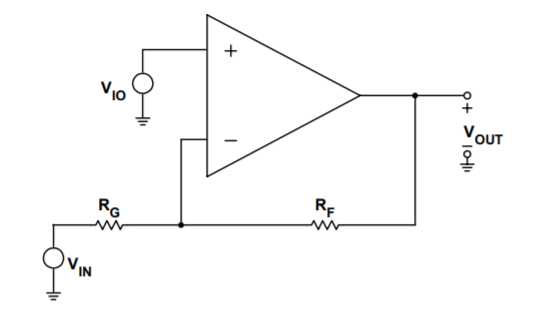
\includegraphics[height=0.2\textheight]{imagenes/vio_amplificacion.png}
	\caption{Modelo de amplificador con configuraci\'on inversora con $V_{IO}$ no despreciable}
	\label{fig:ej_3_efecto_vio}
\end{figure}

El circuito de la figura \ref{fig:ej_3_efecto_vio} representa un amplificador operacional en configuraci\'on inversora con tensi\'on de offset no despreciable modelado por un \textit{op-amp} ideal y una fuente de tensi\'on continua $V_{IO}$. De ignorarse la tensi\'on de offset, puede obtenerse la funci\'on transferencia:

\[\frac{V_{OUT}}{V_{IN}}=\frac{-R_F}{R_G}\]

Sin embargo, si se considera la tensi\'on de offset, no es posible obtener obtener la funci\'on transferencia ya que el sistema no es lineal:

\[V_{OUT}=V_{IN}\frac{-R_F}{R_G} + V_{IO}\left(1+\frac{R_F}{R_G}\right)\]
\[\text{Si }V_{IN} = 0,V_{OUT} = V_{IO}\left(1+\frac{R_F}{R_G}\right) \neq 0 \]
\[\Rightarrow \text{El sistema no es lineal}\]

Dependiendo el orden de $V_{IN}$ y de $V_{IO}$ y de la precisi\'on necesaria, el efecto de $V_{IO}$ en $V_{OUT}$ no puede ser despreciado.

\subsubsection*{Efecto de $I_B^+$ y $I_B^-$}
El amplificador operacional no puede funcionar si se impide el paso de las corrientes de bias. \todo{"impide el paso" suena medio choto pero no s\'e como decirlo m\'as mejor}Si se decide poner un capacitor en serie con una de las entradas, $I_B$ no podr\'a circular, haciendo que el amplificador no funcione correctamente. Ver ejemplo en figura \ref{fig:ej_3_GIC}. \todo{redaccion}

\begin{figure}[htb] %GIC
	\centering
	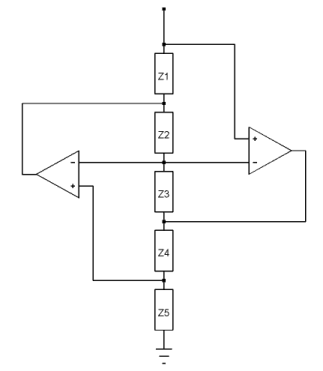
\includegraphics[width=0.35\textwidth]{imagenes/gic.png}
	\caption[Capacitores en un GIC]{Circuito GIC. Si $Z_2$ y $Z_3$ fueran capacitores, no podri\'ian circular las corrientes de bias. Una posible soluci\'on consiste en poner una resistencia en paralelo que permita la circulaci\'on y que sea lo suficientemente grande como para que la impedancia resultante sea aproximadamente capacituva pura.}
	\label{fig:ej_3_GIC}
\end{figure}


Por otro lado, si hay una resistencia $R$ en serie con la entrada del operacional, habr\'a una ca\'ida de tensi\'on $V=I_B^\pm\cdot R$ que puede o no ser despreciable dependiendo de la relaci\'on entre $I_B^\pm$ y $R$ y las caracter\'isticas del circuito. Este efecto es usado en el circuito de medici\'on explicado en la siguiente secci\'on para medir $I_B^+$ y $I_B^-$








\subsection{Circuitos con realimentaci\'on}	\label{ssec:realimentacion}

Un circuito realimentado es aquel en el que una proporcion de la salida se redirige a la entrada con el prop\'osito de controlar el comportamiento del sistema. Se  muestra un diagrama de un sistema realimentado t\'ipico en la figura \ref{fig:ej_3_realimentacion}
\footnote{Es com\'un encontrar el mismo modelo con la diferencia que a la entrada se le resta una se\~nal en vez de sumarse. Ambos modelos pueden representar los mismos sistemas (alcanza con cambiar la fase de $\beta$ en 180$^\circ$ para pasar de uno a otro). En este caso se decidi\'o usar la opici\'on con suma ya que es m\'as simple encontrar la similitud con el circuito analizado (ver siagrama de flujo de sen\~nal en la figura \ref{fig:ej_3_signal_flow_consigna_simplificado}}

\begin{description}
	\item[$A_{OL}$:] ganancia a lazo abierto del sistema (\textit{open-loop})
	\item[$A_{CL}$:] ganancia a lazo cerrado del sistema (\textit{closed-loop})
	\item[$A_{CL\,ideal}$:] ganancia a lazo cerrado ideal del sistema. $lim_{T\rightarrow \infty}A_{CL} = A_{CL\,ideal}$
	\item[$\beta$:] ganancia de realimentaci\'on
	\item[$T=A_{OL}\cdot\beta$:] ganancia de lazo
\end{description}

\begin{figure}[htbp] %diagrama realimentacion
	\centering
	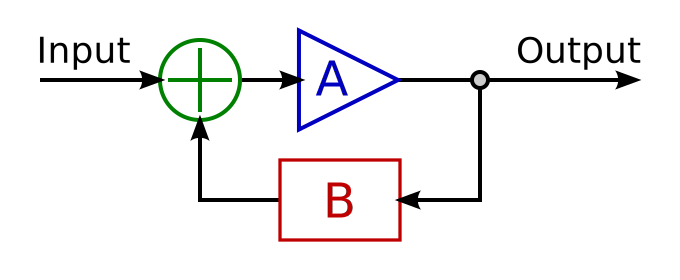
\includegraphics[width=0.5\textwidth]{imagenes/Ideal_feedback_model.png}
	\caption{Diagrama de flujo de se\~nal de sistemas realimentados.}
	\label{fig:ej_3_realimentacion}
\end{figure}


La funci\'on transferencia del sistema H(s) equivale a su ganancia a lazo cerrado:

\[x_d = x_i+x_f\]
\[x_f = \beta x_f\]
\[x_o = A_{OL}x_d = A_{OL}\left( x_i+x_f \right) =  A_{OL}\left( x_i+\beta x_o \right)\]
\[x_o - A_{OL} \beta x_o = A_{OL} x_i\]
\begin{equation}
	\Rightarrow H(s) = A_{CL} = \frac{x_o}{x_i} = \frac{A_{OL}}{1-A_{OL}\beta}
	\label{eq:ej_3_ACL}
\end{equation}

Suponiendo que $T\gg 1$ se obtiene la ganancia a lazo cerrado ideal:
\begin{equation}
	A_{CL\,ideal} = \frac{-1}{\beta}
	\label{eq:ej_3_ACL_IDEAL}
\end{equation}

Un sistema tiene realimentaci\'on negativa si la fase de la ganancia de lazo est\'a entre $180^\circ$ (inclusive) y $360^\circ$ (no inclusive)\todo{googlear algo de esto por que solo lo s\'e porque es palabra santo del senior, no tengo ninguna fuente}, y realimentaci\'on positiva en caso contrario.

\begin{figure}[htbp] %Ejemplo realimentacion negativa y positiva opamp
	\centering
	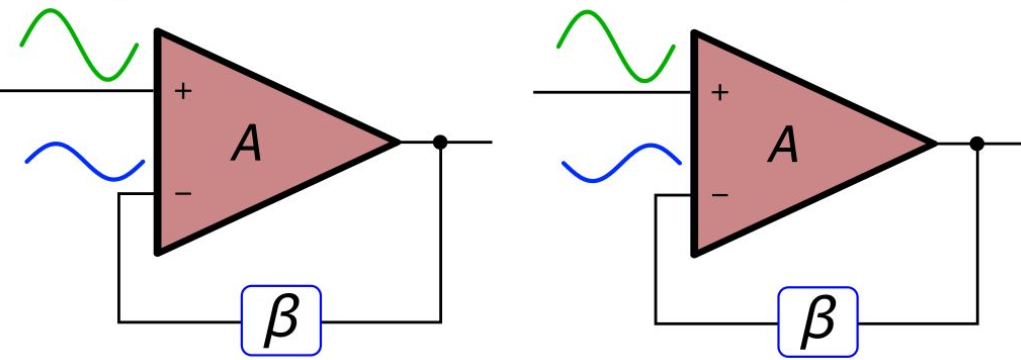
\includegraphics[width=0.5\textwidth]{imagenes/pos_vs_neg_feedback.png}
	\caption{Ejemplo de realimentaci\'on negativa y positiva en un \textit{op-amp}.}
	\label{fig:ej_3_realimentacion_pos_vs_neg_opamp}
\end{figure}










\subsection{Funcionamiento del circuito}
La funci\'on del circuito es medir la tensi\'on de offset y las corrientes de bias. La corriente de bias se obtiene midiendo la ca\'ida de tensi\'on que genera sobre una resistencia de $1M\Omega$. En la tabla \ref{tab:ej_3_datasheet} se observan los valores que se esperan medir.


\begin{table}[htbp]
\centering
\begin{tabular}{ccccccc}
               & \multicolumn{3}{c}{TL081}            & \multicolumn{3}{c}{LF356}    \\
\hline              
               & $V_{IO}$(mV) & $I_B$(pA) & $I_O$(pA) & $V_{IO}$(mV) & $I_B$(pA) & $I_O$(pA) \\
\hline
Valor t\'ipico & 3            & 30        & 5         & 3            & 30    & 3     \\
Valor m\'aximo & 6            & 200       & 100       & 10           & 200   & 50   
\end{tabular}
\end{table}

Todas las tensiones a determinar son amplificadas para as\'i aumentar la precisi\'on en la medici\'on. Una posibilidad ser\'ia amplificar a lazo abierto. Este m\'etodo cuenta con dos desventajas:
\begin{itemize}	%desventajas lazo abierto
	\item La ganancia a lazo abierto $A_{vol}$ t\'ipica de ambos amplificadores es 200V/mV. Con los valores de la tabla \ref{tab:ej_3_datasheet}, el amplificador saturar\'ia.
	\item Incluso si no hubiera saturaci\'on, \todo{redaccion: avol es super impreciso/ cambia una bocha entonces el resultado seria muy impreciso}
\end{itemize}
Por estos motivos se utiliza amplificaci\'on a lazo cerrado. En la figura \ref{fig:ej_3_medicion_vio_simple} se muestra un circuito de medici\'on de $V_{IO}$ con ganancia lazo cerrado. Sabiendo que la ganancia de un circuito de amplificacion no inversor es $1+\frac{R_2}{R_1}$, se obtiene $V_{IO}=\frac{R_1}{R_1+R_2}\cdot V_{OUT}$. 


\begin{figure}[htbp]	%medicion vio simplificado
	\centering
	\begin{subfigure}[t]{0.43\textwidth}
		\centering
		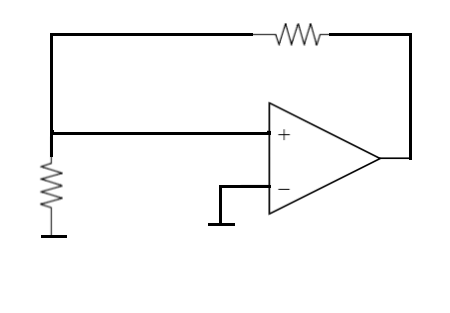
\includegraphics[width=\textwidth]{imagenes/medicion_vio_configuracion_simplificada.png}
		\caption{Con \textit{op-amp} real}
	\end{subfigure}%
	\hfill%%
	\begin{subfigure}[t]{0.43\textwidth}
		\centering
		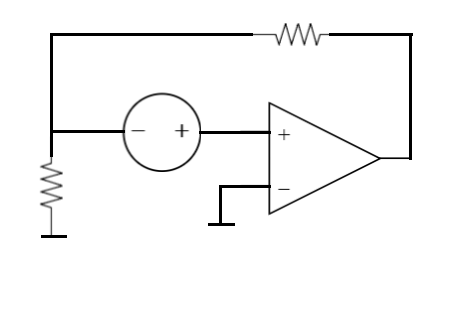
\includegraphics[width=\textwidth]{imagenes/medicion_vio_configuracion_simplificada_opamp_ideal.png}
		\caption{Con \textit{op-amp} ideal y fuente de tensi\'on modelando el \textit{op-amp} real y su tensi\'on de offset}
	\end{subfigure}	
	\caption[Circuito de medici\'on de $V_{IO}$ simplificado.]{Circuito de medici\'on de $V_{IO}$ simplificado.  $V_{OUT} = V_{IO} \cdot \left( 1+ \frac{R_2}{R_1} \right) $. No mide corrientes de bias y amplifica todas las frecuencias por igual.}
	\label{fig:ej_3_medicion_vio_simple}
\end{figure}

Ya que las se\~nales que se quieren medir tienen una amplitud comparable con el ruido que pueda llegar a inducirse en el circuito, es conveniente reducir la amplificaci\'on para las frecuencias mayores a cero. \todo{redaccion} Esto se logra en el circuito presentado en la consigna (figura \ref{fig:ej_3_medicion_vio_consigna})

\begin{figure}[htbp] %medicion vio ib+ ib- posta
	\centering
	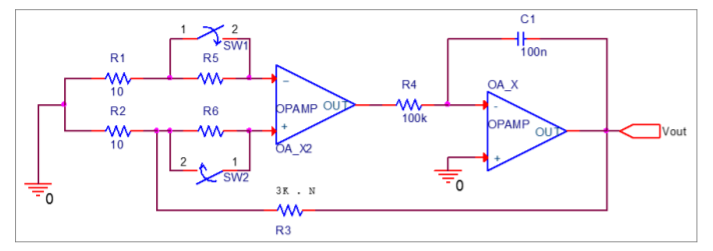
\includegraphics[scale=1]{imagenes/medicion_bias_configuracion_consigna.png}
	\caption{Circuito de medici\'on de $V_{IO}$, $I_B^+$ y $I_B^-$. El dispositivo cuyas caracter\'isticas se miden es el DUT, o \textit{device under test}, el cual es un amplificador con $V_{IO}$ y $I_B$ no despreciables.}
	\label{fig:ej_3_medicion_vio_consigna}
\end{figure}
\todo{grafico de consigna con los valores posta}
\begin{figure}[htbp] %medicion vio ib+ ib- posta con opamp ideal
	\centering
	\missingfigure[figwidth=\textwidth]{circuito con las fuentes}
	\caption{Mismo circuito que en la figura \ref{fig:ej_3_medicion_vio_consigna} cambiando el DUT por el modelo de la figura \ref{fig:ej_3_modelo_opamp_vio_ibias}}
	\label{fig:ej_3_medicion_vio_consigna_modelando}
\end{figure}

Se utiliza un diagrama de flujo de se\~nal (figura \ref{fig:ej_3_signal_flow_consigna_simplificado}) para obtener la funci\'on de transferencia del sistema. Se tomaron la siguiente consideraciones:
\begin{itemize}
	\item $\Delta V_{R1} = I_b^- \cdot 10\Omega \approx 0$
	\item $I_{R2}\approx I_{R3}$
	\item La ganancia a lazo abierto de ambos amplificadores es $A_{vol}$\footnote{Es importante distinguir la ganancia a lazo abierto de un \textit{op-amp} $A_{vol}$ de la ganancia a lazo abierto del circuito total $A_{OL}$ }
\end{itemize}


\begin{figure}[htpb]%signal flow consigna
	\centering
	\begin{subfigure}[t]{0.49\textwidth}
		\centering
		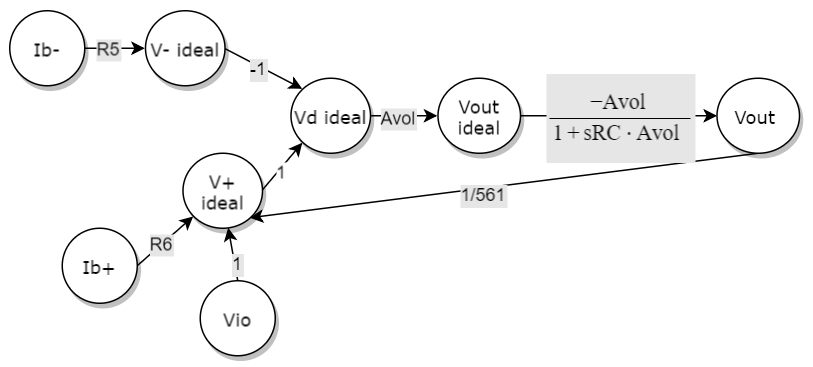
\includegraphics[width=\textwidth]{imagenes/signal_flow_consigna.png}
		\caption{Diagrama de flujo de se\~nal para el circuito de la consigna usando el modelo de la figura para el DUT}
		\label{fig:ej_3_signal_flow_consigna_no_simplificado}
	\end{subfigure}%
	\hfill%%
	\begin{subfigure}[t]{0.49\textwidth}
		\centering
		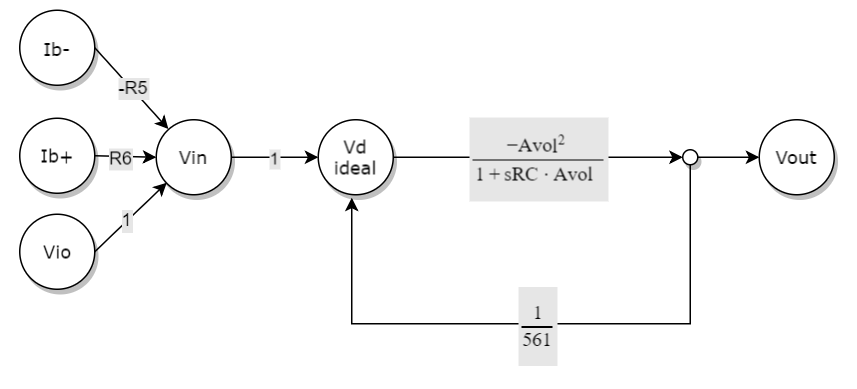
\includegraphics[width=\textwidth]{imagenes/signal_flow_consigna_simplificado.png}
		\caption{Simplificaci\'on del diagrama de flujo de se\~nal. La estructura coincide con la de un circuito con realimentacion (ver figura \ref{fig:ej_3_realimentacion}). }
		\label{fig:ej_3_signal_flow_consigna_simplificado}
	\end{subfigure}
	\label{fig:ej_3_signal_flow_consigna}	
\end{figure}


El diagrama de flujo de se\~nal coincide con el de un sistema realimentado descripto en la secci'on \ref{ssec:realimentacion}. La \'unica diferencia es que en este caso la entrada no es una \'unica se\~nal sino una suma:

\begin{equation}
	V_{in} = V_{IO} + I_B^+\cdot R6 - I_B^-\cdot R5
	\label{eq:ej_3_vin_aparente}
\end{equation}

Cabe destacar $V_{in}$ es una forma abstracta de agrupar los efectos generados por tres se\~nales reales distintas, y no corresponde necesariamente con una diferencia de potencial real entre dos puntos.

 Se puede obtener entonces la ganancia de lazo cerrado y la ganancia de realimentaci\'on del circuito:
\[\beta = \frac{1}{561}\]
\[A_{OL} = -\frac{A_{vol}^2}{1+sRC\cdot A_{vol}}\]

Con estos valores y teniendo en cuenta la ecuaci\'on \ref{eq:ej_3_ACL} se obtiene la funci\'on transferencia del sistema:

\begin{equation}
	H(s)=\frac{-\frac{A_{vol}^2}{1+sRC\cdot A_{vol}}}{1+\frac{A_{vol}}{1+sRC\cdot A_{vol}}\beta}
	=-\frac{1}{\frac{1}{A_{vol}^2}+\beta}\cdot \frac{1}{\frac{s}{\frac{1+A_{vol}^2\beta}{RCA_{vol}}} +1}
	\label{eg:ej_3_transferencia_consigna_sin_simplificar}
\end{equation}


Si se considera que $A_{vol}^2\beta \gg 1 \Rightarrow \beta \gg \frac{1}{A_{vol}^2}$ se puede simplificar la expresi\'on:


\begin{equation}
	H(s) = -\frac{1}{\beta}\cdot \frac{1}{\frac{s}{\frac{A_{vol}\beta}{RC}}+1}
	\label{eq:ej_3_transferencia_consigna_simplificada}
\end{equation}


Sabiendo que $lim_{T\rightarrow \infty}A_{CL} = A_{CL\,ideal}$:

\begin{equation}
	A_{CL\,ideal} = -\frac{1}{\beta} = -561
\end{equation}


\subsubsection{Funcionamiento en DC: mediciones de $V_{IO}$ y $I_B$}

Cuando $f=0$, evaluando en la funci\'on transferencia (ecuaci\'on \ref{eg:ej_3_transferencia_consigna_sin_simplificar}) se obtiene que la ganancia del circuito es $-\frac{1}{\beta}=-561$, por lo que $V_{in}=-\frac{V_{out}}{561}$


\begin{description}
	\item[Medici\'on de $V_{IO}$:] Cortocircuitando las resistencias R5 y R6 se obtiene que $V_{in} = V_{IO}$, valor que se puede obtener midiendo $V_{OUT}$:
	
	\[V_{IO} = -\frac{V_{OUT}}{561}\]
	\item[Medici\'on de $I_B^\pm$ y $I_B$:] Cortocircuitando R5 se obtiene $-\frac{V_{OUT}}{561} = V_{IO} + I_B^+\cdot R6$. Despejando:
	\[I_B^+=\frac{1}{R6}\cdot\left( -\frac{V_{OUT}}{561}-V_{IO}  \right) \]
	An\'alogamente,
	\[I_B^-=-\frac{1}{R5}\cdot \left( V_{IO} + \frac{V_{OUT}}{561}   \right)\]
	Una vez obtenidas $I_B^\pm$, se calcula $I_B$ definida como $\frac{I_B^++I_B^-}{2}$
\end{description}

\begin{table}[htbp]
\centering
\begin{tabular}{ccccc}
                       & \multicolumn{2}{c}{TL081} & \multicolumn{2}{c}{LF356} \\
\hline
Par\'ametro a calcular & $V_{OUT}$(mV)& Resultado  & $V_{OUT}$(mV)& Resultado  \\
\hline
$V_{IO}$               & 255          & -0,455mV   & 135          & -0,241mV   \\
$I_B^+$                & 0,675        & 453pA      & 0,179        & 241pA      \\
$I_B^-$                & 202          & -94,5pA    & 207          & -143pA     \\
$I_{IO}$			   &     ---      & 584 pA	   &	  ---     & 384pA      \\
$I_B$				   &     ---      & 179 pA     &      ---     & 49pA
\end{tabular}%

\caption{Resultados}
\label{tab:ej_3_resultados}
\end{table}

Las mediciones que son acordes a lo especificado en la hoja de datos son $V_{IO}$  y $I_B$ en los dos amplificadores. Por otro lado, se midieron valores de $I_O$ mayores al m\'aximo especificado por el fabricante, tambi\'en en los dos casos.



\subsubsection{Funcionamiento en AC}























\subsection{Estabilidad en diferentes configuraciones}




La estabilidad del sistema se analiza viendo la posici\'on de los polos en el plano complejo


En la figura \ref{fig:ej_3_realimentacion_pos_vs_neg_opamp} se muestran ejemplos de realimentaci\'on negativa y positiva en un amplificador operacional.



\subsubsection{Consigna}
\subsubsection{Uno invertido}
\subsubsection{Ambos invertidos}












\subsection{Medici\'on de $V_{IO}$ y $I_B^\pm$}


\begin{itemize}
	\item estabilidad
	\item inversion de los opamps
\end{itemize}

\end{document}


%


%


%\documentclass[../../main.tex]{subfiles}

\usepackage{gensymb}
\usepackage{textcomp}
\usepackage[colorlinks=true]{hyperref}

\begin{document}
\
\section{Sensor de Temperatura}

\subsection{Introducción}

Se implementará un sensor de temperatura utilizando el circuito integrado LM35, un circuito integrado cuya tensión de salida varía linealmente con la temperatura. \par
Según la datasheet del integrado mencionado anteriormente del fabricante Texas Instruments ''LM35 Precision Centigrade Temperature Sensors'', con última revisión en diciembre de 2017, el integrado ofrece un rango de medición asegurada de entre -55\celsius y 150\celsius, con una variación de 10mV/\celsius, siendo el 0\celsius correspondiente a 0V. \par
Se busca implementar a partir de estos valores, un sensor de temperatura capaz de medir con máxima excursión entre 35°C y 45°C, con 0V correspondiendo a 35\celsius y 5V a 45\celsius.\par
A partir del circuito se podrá utilizar un conversor analógico-digital para lograr manipular la información de temperatura como se requiera. \par
Se tuvo como prioridad minimizar la cantidad de componentes utilizados, garantizar la confiabilidad y precisión de los valores que el circuito devuelva. Se tuvo en cuenta la protección del circuito receptor de la señal, haciendo que la señal de salida no sobre pase el intervalo [-1;6] volts.

\subsection{Análisis del LM35 y condiciones a tener en cuenta}
\label{condiciones} 	%marker para link a esta seccion

Según la datasheet mencionada anteriormente, deben mencionarse ciertas consideraciones a tener en cuenta: 
\begin{itemize}
\item El error máximo del LM35 para medir temperatura es de 0.5\celsius, por lo que el circuito derivado a partir de él no podrá asegurar un error menor a este mismo.
\item La tensión de alimentación para el LM35 será de entre -0.2 V y 35 V como valores máximos, 4V  y 30 V como valores típicos.
\item La máxima temperatura de juntura es 150\celsius, la cual no se contradice con el rango de valores elegidos para el circuito implementado. La máxima temperatura de juntura es la máxima temperatura que la juntura del semiconductor interno puede tolerar manteniendo al LM35 en estado operativo.
\item La corriente de entrada del LM35 será baja, de 60$\mu$A máximo.
\item La corriente de salida del LM35 tomará un valor máximo de 10mA.
\item El LM35 tiene una impedancia de salida baja, de 0.1$\ohm$.
\end{itemize}

Es importante hacer notar que una baja impedancia de salida se corresponde con un circuito emisor de señal como es el caso de un sensor de temperatura. Esto es así porque si la señal emitida en tensión deberá ser recibida por otro circuito que interpretará o modificará la señal recibida, y si la impedancia de entrada del circuito receptor fuera más baja que la de salida del emisor, entonces
siendo z1 la impedancia de salida del emisor y z2 la impedancia de entrada del receptor, por divisor de tensión:
$V_o$ = $\frac{z_{2}}{z_{1}\text{+}z_{2}}$ $V_i$\par
Donde $V_i$ es la tensión de entrada y $V_o$ la de salida. Si se asume que la potencia se mantiene constante en el traspaso entre los dos circuitos, se aprecia de aquí que si |z1|«|z2| y 1«|z2|, entonces $\frac{z_{2}}{z_{1}\text{+}z_{2}}\approx 1$, con lo cual la tensión de salida del circuito emisor original sería equivalente a la tensión de entrada del circuito receptor, por lo que la señal sería recibida correctamente en valor. \par
Es por esto que se intentará obtener una impedancia de entrada de nuestro circuito adaptador mucho mayor a la impedancia de salida de 0.1$\ohm$ del LM35.

\subsection{Cambio de rango operacional}

El comportamiento del LM35 puede ser representado matemáticamente con una transformación lineal de grados celsius a tensión en volts\par 
$TL_{35}$: c$\epsilon$ [-55; 150] -> v$\epsilon$[-0.55; 1.5] / $TL_{35}$(c) = 0.01$\cdot$c. 
El circuito a implementar pretende utilizar una transformación lineal\par
$TL_{cambio}$: $v_1\epsilon$ [0.35;0,45] -> $v_2\epsilon$ [0;5] de forma tal que 
$TL_{cambio}(TL_{35}(c))= TL_{sensor}(c)$ donde $TL_{sensor}: c\epsilon [0.35;0,45] -> v_2\epsilon[0;5]$ será la transformación total del circuito.

Así, se deberá resolver el siguiente sistema de ecuaciones:

	 \begin{equation}
  	   \left\{
	  	    \begin{array}{ll}
		 					0 = m\mathrm{\cdot}0.35 + b \\
			 				5 = m\mathrm{\cdot}0.45 + b \\
	     	 \end{array}
	     	\right.
 	\end{equation}

Que tiene como solución m=50 $\cap$ b = -17.5.

Para realizar la transformación lineal sobre la salida del LM35, se decidió utilizar un opamp con realimentación negativa, dispuesto de la siguiente manera:

\begin{figure}[H]	%y = mx +b en circuito
	\centering
	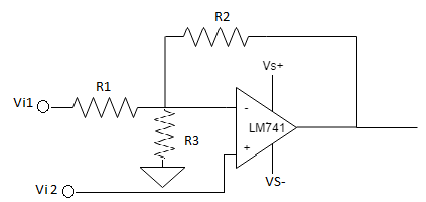
\includegraphics[scale=1.3]{imagenes/adder.png}
	\caption{Cambio de rango operacional en circuito}
	\label{fig:ej6_adder}
\end{figure}

El cual se resolverá por superposición (suponemos que el opamp está operando en su zona lineal) para mostrar que cumple con la necesidad de la multiplicación y la resta necesarias:
\begin{itemize}
\item Pasivamos la fuente Vi1, dejando un no inversor:
\begin{figure}[H]	%vi1 pasivada
	\centering
	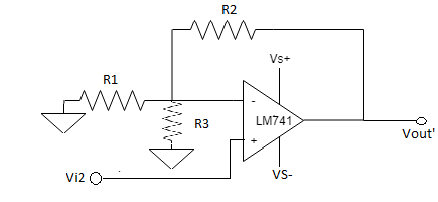
\includegraphics[scale=1.3]{imagenes/adder_pasivo_vi1.png}
	\caption{Vi1 pasivada}
	\label{fig:ej6_adder_pasivo_vi1}
\end{figure}
Entonces Vout' = $(1+\frac{R2(R1+R3)}{R1R3})\cdot$Vi2

\item Pasivamos la fuente Vi2, dejando un inversor:
\begin{figure}[H]	%vi2 pasivada
	\centering
	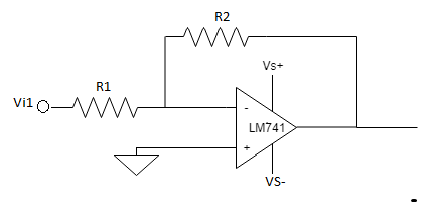
\includegraphics[scale=1.3]{imagenes/adder_pasivo_vi2.png}
	\caption{Vi2 pasivada}
	\label{fig:ej6_adder_pasivo_vi2}
\end{figure}

Entonces Vout'' = $-\frac{R2}{R1}\cdot$Vi1
\item Obtenemos la salida como la superposición de los dos estados calculados anteriormente:\par
Vout = Vout' + Vout'' = $(1+\frac{R2(R1+R3)}{R1R3})\cdot$Vi2 $-\frac{R2}{R1}\cdot$Vi1\par

Si Vi1 es una entrada continua positiva de valor Vs+ y Vi2 es la salida del LM35, entonces, para cumplir con y = mx + b y la solución al sistema de ecuaciones mencionada anteriormente: \par
	 \begin{equation}
  	   \left\{
	  	    \begin{array}{ll}
		 					50 = 1+\mathrm{\frac{R2(R1+R3)}{R1R3}}\\
			 				-17,5 = \mathrm{-\frac{R2}{R1}\cdot}Vs+ \\
	     	 \end{array}
	     	\right.
 	\end{equation}

 	
 	Por lo que como Vs+ será la alimentación del LM35 y dados los requerimientos del mismo se podrá alimentar en el rango recomendado con cualquier valor de tensión de entre 4V y 30V, si se elige Vs+ = 12V, \par

 	Y el sistema queda 

\end{itemize}
\subsection{Protección del circuito a conectar}

Dado que el nuevo sensor a implementar será utilizado para alguna aplicación en concreto, deberá ser conectado a un segundo circuito ''receptor'' que utilice la información de la temperatura actual, por ejemplo un conversor analógico-digital. Es por esta razón que se prohibirán tensiones de salida que puedan resultar peligrosas para el receptor. Se garantiza que la salida, por ende, no será superior a 6V ni inferior a -1V. \par
Para lograr lo anterior, se utilizará un diodo Zener, que hará clipping asimétrico a la señal de salida (ver pedal de distorsión o ej5 para mayor información sobre clipping).\par
Los \underline{diodos Zener} suelen usarse para protección de circuitos y pueden ser representados por su curva característica:

\begin{figure}[H]	%curva diodo zener
	\centering
	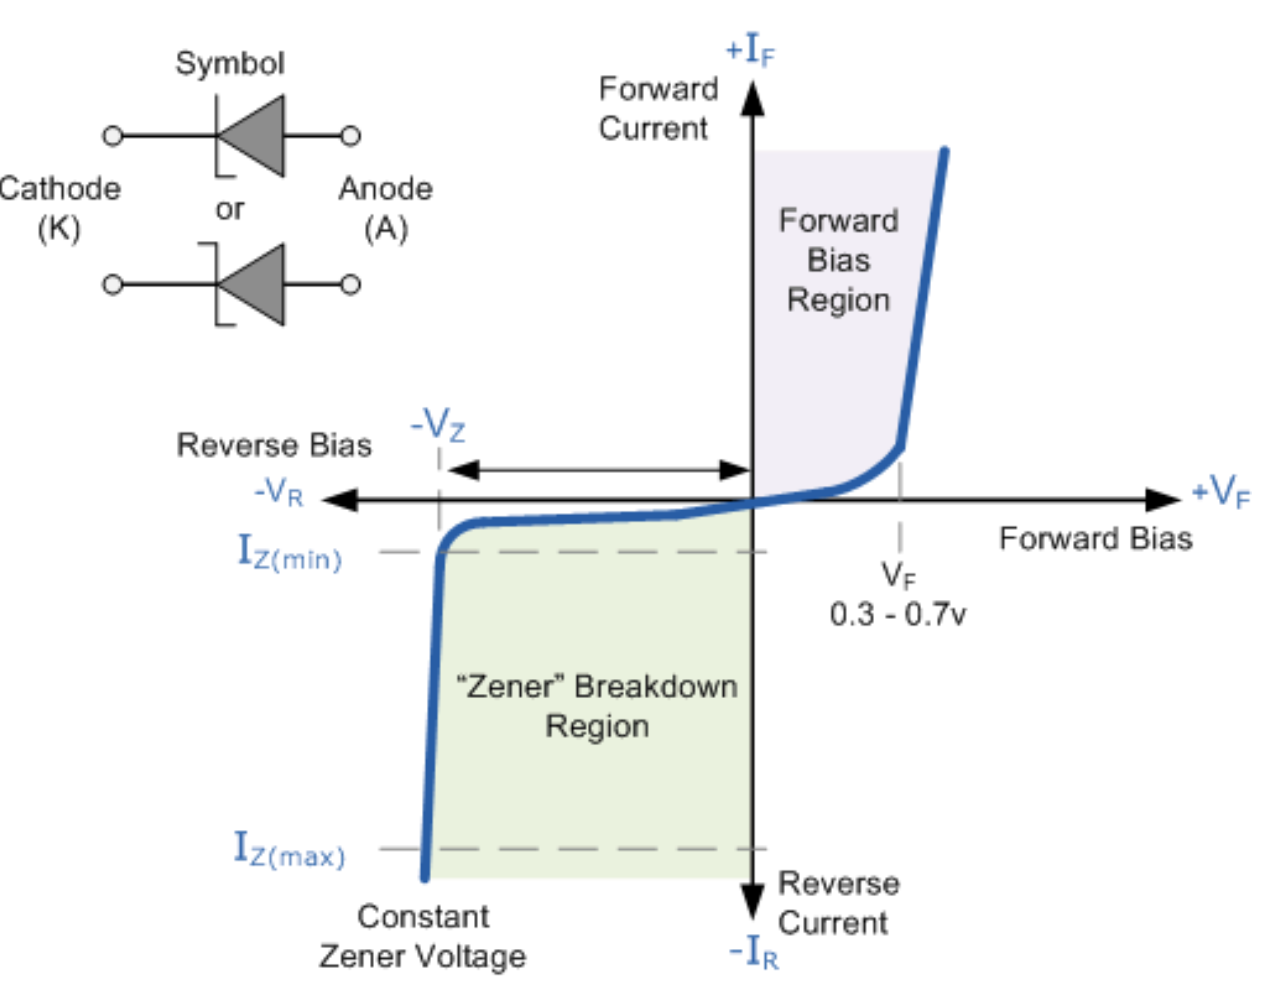
\includegraphics[scale=0.5]{imagenes/zener_diode_curva.png}
	\caption{Curva característica del diodo Zener}
	\label{fig:ej6_zener_diode_curva}
\end{figure}

De esta curva se hace notar que al superar el valor de tensión $V_f$ o al llegar a un nivel de tensión menor a $V_z$, la demanda de corriente por parte del diodo aumentará exponencialmente. Es aquí cuando recordamos una de las condiciones de la subsección \nameref{condiciones}: La corriente de salida del LM35 tomará un valor máximo de 10mA. Esto deberá ser tenido en cuenta cuando se presente la implementación final del circuito. \par
De esta manera, se buscará que los valores de $V_f$ y $V_z$ sean tales que la demanda de corriente sea tan alta luego de los mismos que la tensión tenga que caer a estos valores para que se logre suplir. De esta manera, se muestra gráficamente la tensión de salida en función de la tensión de entrada:

\begin{figure}[H]	%curva diodo zener
	\centering
	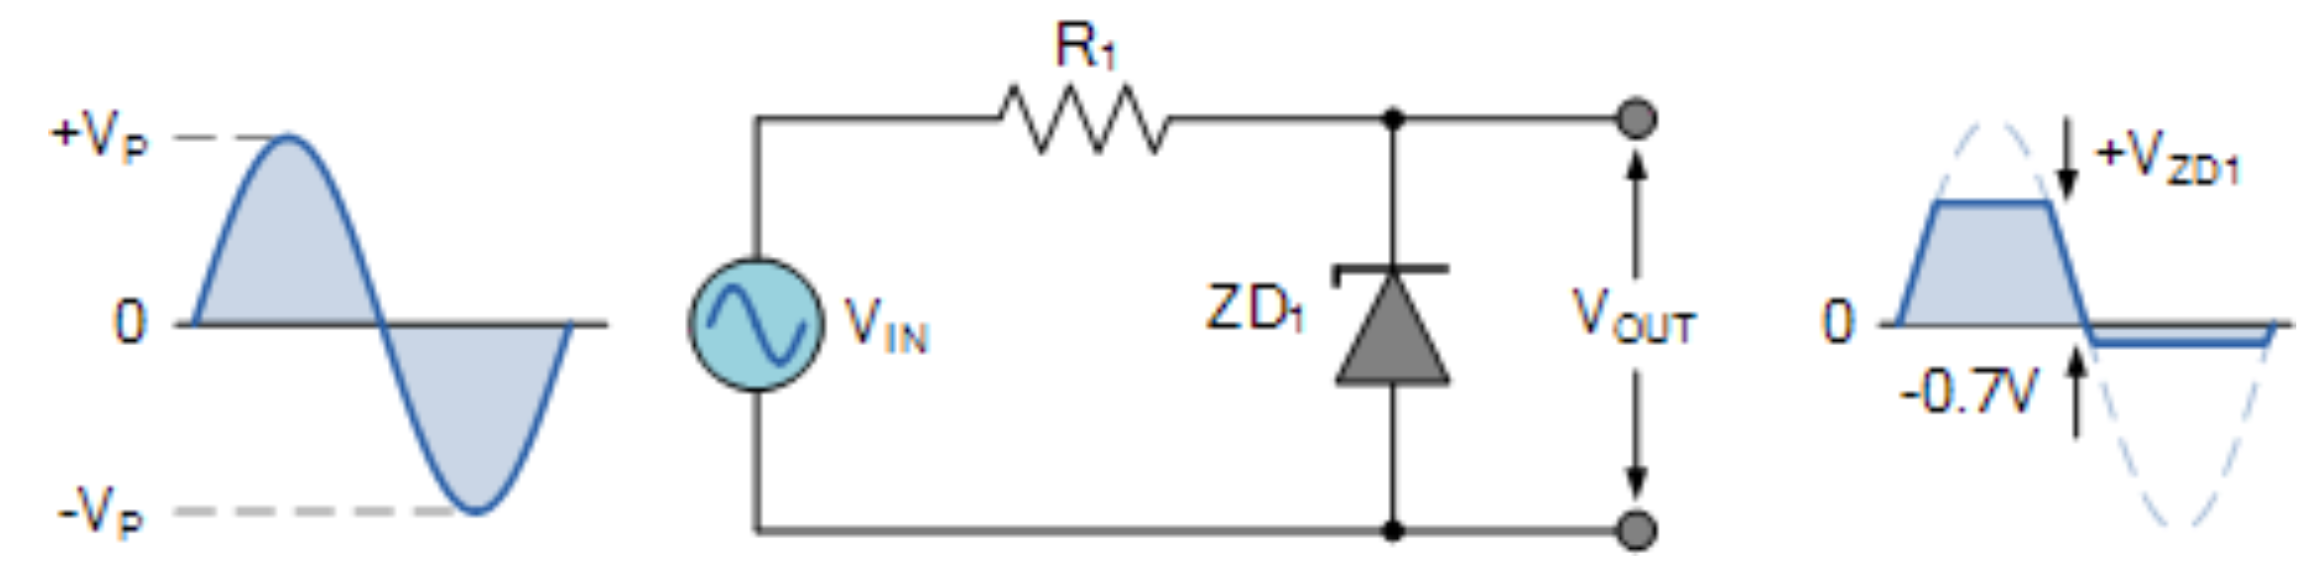
\includegraphics[scale=0.5]{imagenes/zener_diode_efecto.png}
	\caption{Efecto del diodo Zener sobre la entrada}
	\label{fig:ej6_zener_diode_efecto}
\end{figure}

Así es como se observa que $V_f$ = -0.7V y $V_z$$\approx$6V. Cabe destacar que el valor de $V_z$ es aproximado a 6V porque el valor no podrá ser excedido en absoluto como restricción de protección, por lo que $V_z<6V$.

\subsection{Implementación del circuito}


\end{document}

\end{document}
